\chapter{Причинность, восстановление графов, цепи Маркова и HMM}
\label{ch:causality}

Корреляция не доказывает причинность. Парадокс Симпсона показывает, как маргинальная связь исчезает или меняет знак при учёте смешивающей переменной.
Причинные графы (DAG) формализуют направленные механизмы и правила интервенций \citep{pearl2009}. Марковские модели описывают последовательности с памятью на один (или несколько) шагов. Скрытые марковские модели (HMM) \citep{bishop2006} разделяют наблюдаемый сигнал и латентное состояние~--- основа распознавания речи, разметки частей речи и биоинформатики.


На протяжении главы полезно возвращаться к трём вопросам из предисловия: постановка и допущения; применимость процедуры и графики; размер эффекта и альтернативные объяснения. Корреляция не заменяет причинный граф. 
В гл.~\ref{ch:regression} мы оценивали линейные связи $X\to Y$ и интерпретировали коэффициенты при условии, что модель корректно специфицирована. В гл.~\ref{ch:hypothesis} проверяли наличие эффекта по p-value и доверительным интервалам.
Здесь вопрос ставится иначе. Что именно означает эффект и какие переменные нужно учитывать при его оценке?
Регрессия с дополнительными предикторами~--- частный случай условной зависимости. Причинный анализ объясняет, когда такое стратифицирование восстанавливает истинный механизм, а когда создаёт ложную картину.
Марковские цепи и HMM, в свою очередь, переносят идею условной независимости на последовательности. Будущее зависит от прошлого только через настоящее~--- прямой аналог d-разделимости во времени.

\section{Парадокс Симпсона}

\begin{definition}
Парадокс Симпсона~--- ситуация, когда агрегированная и стратифицированная по подгруппам зависимость между $X$ и $Y$ имеют противоположный знак или разную интерпретацию.
\end{definition}

Классический пример~--- клиническое исследование лекарства от холестерина.
В агрегате плацебо кажется эффективнее (83\% выздоровлений против 78\%), но в каждой подгруппе лекарство лучше на 4--5\%.
Интуитивно кажется, что детализация не может ухудшить вывод, но парадокс Симпсона показывает обратное. Агрегация и стратификация отвечают на разные вопросы.
Маргинальное сравнение смешивает подгруппы с разной базовой частотой исхода и разной долей получивших лечение. Условное сравнение внутри гомогенных групп может дать противоположный знак эффекта.
Тот же механизм лежит в основе споров об эффекте регрессии к среднему и о неверной интерпретации частичных коэффициентов без причинной схемы.

Пример~1 (смешивающий фактор~--- пол $Z$).
\begin{center}
\small
\begin{tabular}{lrrr}
\toprule
 & лекарство & плацебо & \\
\midrule
всего.& 78\% & 83\% & плацебо лучше \\
мужчины.& 93\% & 87\% & лекарство лучше \\
женщины.& 73\% & 69\% & лекарство лучше \\
\bottomrule
\end{tabular}
\end{center}
Причина. Пол влияет и на назначение лечения, и на исход. В выборке больше женщин получили лекарство, а у женщин исход хуже.

Пример~2 (медиатор~--- давление $Z$). Те же маргинальные цифры, но стратификация по конечному давлению (пост-лечение) вновь показывает преимущество лекарства в каждой группе.
Здесь $X\to Z\to Y$. Давление~--- следствие лечения, а не смешивающий фактор. Условие на $Z$ блокирует причинный путь $X\to Y$ и открывает ложный путь через $X\leftarrow U\to Y$ (если $U$ есть).
Нельзя автоматически доверять более детальной стратификации. Всё зависит от того, как переменная разбиения связана с $X$ и $Y$ в причинном графе.
Смешивающий фактор нужно учитывать. Посредник и коллайдер~--- осторожно.

Пример лекарства и пола. Маргинально плацебо лучше, в подгруппах~--- лекарство лучше.
Без DAG легко спорить, какая таблица корректна. С DAG ясно, что пол~--- смешивающий фактор, и корректировка по $Z$ восстанавливает ACE, тогда как медиатор (давление) требует другой формулы.
Парадокс Симпсона~--- мост между $\chi^2$/регрессией (гл.~\ref{ch:anova},~\ref{ch:regression}) и do-исчислением.

\section{Причинные графы}

\begin{definition}
DAG~--- направленный ациклический граф. Вершины~--- переменные, рёбра $X\to Y$~--- прямое влияние $X$ на $Y$.
Путь через заднюю дверь (ПЗД) от $X$ к $Y$ начинается ребром $X\leftarrow$ и заканчивается $\to Y$.
\end{definition}

Три типичных паттерна.
\begin{itemize}
    \item Цепочка $X\to Y\to Z$. $X$ и $Z$ зависимы, но
          $X\perp Z\mid Y$ (пример. бюджет школы $\to$ средний балл $\to$ доля поступающих в ВУЗы).
    \item Вилка $Y\leftarrow X\to Z$. $Y$ и $Z$ зависимы, но
          $Y\perp Z\mid X$ (пример. продажи мороженого, температура, число преступлений).
    \item Коллайдер $Y\to X\leftarrow Z$. $Y\perp Z$, но
          $Y\not\perp Z\mid X$ (пример. выбор ведущего, игрока и положение приза в задаче Монти-Холла).
\end{itemize}
Цепочка объясняет, почему лишний предиктор $Y$ может ослабить связь $X$ с $Z$ в регрессии. Вилка~--- почему $Y$ и $Z$ коррелируют без прямой связи. Коллайдер~--- почему отбор по $X$ (например, только лучшие кандидаты) создаёт ложную ассоциацию между $Y$ и $Z$.

d-разделимость. Множество $Z$ блокирует путь, если на каждом неколлайдерном сегменте $A\to M\to C$ или $A\leftarrow M\to C$ вершина $M\in Z$, а каждый коллайдер $A\to M\leftarrow C$ не в $Z$ и не имеет потомков в $Z$.
Если $Z$ блокирует все пути $X\leadsto Y$, то $X$ и $Y$ d-разделены условно на $Z$. При марковском факторизации это эквивалентно $X\perp Y\mid Z$.

Графическое правило d-разделимости заменяет перебор всех подмножеств $Z$ при проверке условной независимости. Достаточно нарисовать DAG и пройти по путям.
На практике экспертная или литературная схема задаёт кандидатов на набор для корректировки. Статистика (регрессия, IPW) лишь оценивает эффект при выбранном множестве.
Ошибка в графе~--- систематическая ошибка вывода, которую не исправит увеличение выборки. Это контраст с обычной асимптотикой МНК (гл.~\ref{ch:regression}).
Три паттерна (цепочка, вилка, коллайдер) покрывают большинство ошибок корректировки. Включение посредников блокирует путь $X\to Y$. Условие на коллайдер открывает ложный путь. Игнорирование смешивающего фактора смещает ACE.
Рисуя DAG до регрессии, исследователь явно перечисляет, какие переменные войдут в $X$, а какие~--- нет.

\section{Интервенции и do-исчисление}

\begin{definition}
Do-оператор $do(X=x)$~--- хирургия графа. Удаляются все входящие в $X$ рёбра, затем $X$ фиксируется в $x$.
Средний каузальный эффект (ACE) определяется как
\[ ACE = P(Y=y_1\mid do(X=x_1)) - P(Y=y_1\mid do(X=x_0)).
\]
\end{definition}

Пример~1 ($Z$~--- пол, смешивающий фактор). Граф $Z\to X$, $Z\to Y$, $X\to Y$. После $do(X)$.
\[ P(Y=y\mid do(X=x)) = \sum_z P(Y=y\mid X=x,Z=z)\,P(Z=z).
\]
Формула~--- стандартная корректировка по смешивающему фактору. Мы взвешиваем условные исходы по распределению $Z$ в населении, а не среди наблюдаемых групп лечения.
Численно. $P(\text{выздор.}\mid do(\text{лекарство}))=0{,}832$, $P(\text{выздор.}\mid do(\text{плацебо}))=0{,}782$ $\Rightarrow$ $ACE=+0{,}05$ (лекарство полезно).

Пример~2 ($Z$~--- давление, медиатор). Граф $X\to Z\to Y$, $X\to Y$. Оперированный граф совпадает с наблюдаемым по $Y$. $P(Y\mid do(X))=P(Y\mid X)$, $ACE=-0{,}05$ (маргинально плацебо лучше, хотя в подгруппах по $Z$~--- наоборот).

Критерий задней двери (KЗД). Множество $Z$ удовлетворяет KЗД для $(X,Y)$, если
\begin{enumerate}
    \item $Z$ не содержит потомков $X$;
    \item $Z$ блокирует все пути $X\leadsto Y$, содержащие $X\leftarrow$.
\end{enumerate}
Тогда
\[ P(y\mid do(x))=\sum_z P(y\mid x,z)\,P(z).
\]
Обратное вероятностное взвешивание.\[ P(y\mid do(x))=\sum_z \frac{P(x,y,z)}{P(x\mid z)}.
\]
Знаменатель $P(x\mid z)$~--- балл включения.

Критерий передней двери (КПД). Медиатор $M$ удовлетворяет КПД, если перекрывает все направленные пути $X\to Y$, нет незакрытых ПЗД из $X$ в $M$, и все ПЗД из $M$ в $Y$ блокируются $X$. Тогда
\[ P(y\mid do(x))=\sum_m P(m\mid x)\sum_{x'}P(y\mid x',m)\,P(x').
\]
Курение и рак (КПД). Скрытый генотип $U$ смешивает $X$ (курение) и $Y$ (рак). Маргинально курильщики болеют реже (15\% против 90\%), но стратификация по смоле $Z$ (медиатор $X\to Z\to Y$) показывает вред курения в обеих подгруппах.
Формула передней двери восстанавливает $P(y\mid do(x))$ без наблюдения $U$.
Условная регрессия на коллайдере открывает ложный путь (M-смещение).
В KЗД нельзя включать потомков $X$ и коллайдеры на пути $X\to Y$.
Причинность по Грейнджеру ($X$ причинно влияет по Грейнджеру на $Y$, если прошлое $X$ улучшает прогноз $Y$) не равна структурной причинности при скрытых общих факторах.

Расчёт ACE для лекарства. Маргинальная разность исходов может иметь знак, противоположный $ACE=+0{,}05$ после корректировки по полу.
Численно важно не только значимо/не значимо, а как меняется оценка при разных наборах для корректировки. Анализ чувствительности по допустимым смешивающим факторам обязателен в прикладных отчётах.

\section{Восстановление графа из данных}

Алгоритм PC (индуктивная причинность). Вход.~--- множество вершин $V$. Выход~--- частично ориентированный DAG.
\begin{enumerate}
    \item Скелет. Для каждой пары $(A,B)$ найти наименьшее
          $S_{AB}$, такое что $A\perp B\mid S_{AB}$ (тесты условной независимости). Если не найдено~--- ребро $A\text{---}B$.
    \item v-структуры. Для несмежных $A,B$ с общим соседом
          $C$. Если $C\notin S_{AB}$, ориентировать $A\to C\leftarrow B$.
    \item Правила Meek (до насыщения). Если $A\to B\text{---}C$
          и $A$, $C$ не смежны, то $B\to C$. Если $A\to B\to C$ и $A\text{---}C$, то $A\to C$. И т.д.
\end{enumerate}
На практике перебор $S_{AB}$ экспоненциален. Используют эвристики ограничения порядка и размера $S_{AB}$.
Идея PC проста. Нет ребра эквивалентно найденному CI. Есть ребро~--- не удалось разделить.
Ориентация v-структур опирается на асимметрию. Коллайдер $A\to C\leftarrow B$ не разделяет $A$ и $B$ маргинально, но разделяет при условии на других соседей. Отсутствие $C$ в минимальном $S_{AB}$~--- сигнал для стрелок в $C$.
Правила Meek доводят частичный граф до максимально ориентированного DAG без противоречий.

\begin{center}
\footnotesize
\begin{tabularx}{\linewidth}{|>{\raggedright\arraybackslash}X|>{\raggedright\arraybackslash}X|>{\raggedright\arraybackslash}X|}\hline
Признаки & дискретные & непрерывные \\\hline
Распределение & мультиномиальное & нормальное \\\hline
Тест CI & $\chi^2$ (таблицы сопряжённости) & частная корреляция Стьюдента \\\hline
Критерий графа & \multicolumn{2}{c|}{BIC} \\\hline
\end{tabularx}
\end{center}

Синтетические данные с графом $X\to Z\to Y$ иллюстрируют восстановление. Маргинально $X$ и $Y$ коррелированы, условно на $Z$~--- нет (цепочка).
PC находит рёбра $X\text{---}Z\text{---}Y$ и ориентирует $X\to Z\to Y$.

Важное ограничение. Из данных без эксперимента восстанавливается класс эквивалентных DAG (класс марковской эквивалентности). v-структуры и скелет идентифицируются при условии верности графа, но направление некоторых рёбер остаётся неопределённым.
Поэтому PC в задаче об авиабилетах (гл.~\ref{ch:labs}) дополняют экспертным графом и сравнением ACE при разных наборах для корректировки.

Причинность по Грейнджеру. Между рядами $x_t$ и $y_t$ существует причинность Грейнджера $x\to y$, если дисперсия ошибки прогноза $\hat y_{t+1}$ по $(y_1,\ldots,y_t,x_1,\ldots,x_t)$ меньше, чем только по прошлому $y$.
Это операциональное определение. $X$ помогает предсказать $Y$. Оно совпадает с причинностью только если в VAR включены все смешивающие факторы и порядок лагов адекватен (см.~гл.~\ref{ch:timeseries}).

VAR-модель.\[ y_t = \alpha + \sum_{i=1}^{k_1}\phi_{1i} y_{t-i} + \sum_{i=1}^{k_2}\phi_{2i} x_{t-i} + \varepsilon_t.
\]
Порядки $k_1,k_2$~--- по AIC/BIC. $H_0\colon\phi_{21}=\cdots=\phi_{2k_2}=0$. Статистика
\[ F = \frac{(RSS_r-RSS_{ur})/k_2}{RSS_{ur}/(T-k_1-k_2-1)} \sim F_{k_2,\,T-k_1-k_2-1}.
\]
Многомерный случай. Добавляют лаги всех остальных рядов $z^j_t$. При большом числе признаков~--- lasso/ridge для отбора лагов.
Граф строят по парам с значимым $F$ с поправкой на множественные сравнения.

PC-алгоритм и причинность Грейнджера~--- два края спектра. Первый ищет структуру через CI-тесты (слабая мощность при малом $n$, см.~гл.~\ref{ch:multiple}). Второй~--- предсказуемость во времени (гл.~\ref{ch:timeseries}).
На практике их комбинируют с экспертным DAG и анализом чувствительности наборов для корректировки.
PC и Грейнджер отвечают на разные вопросы. Какие CI выполняются? Помогает ли прошлое $x$ предсказать $y$?
Пример $X\to Z\to Y$. PC находит скелет и ориентирует v-структуру. Грейнджер может показать $x\to y$ при лагах, даже если $Z$ не включён в VAR~--- смешивание остаётся.
Комбинация экспертного DAG, PC и временных тестов~--- практический стандарт, а не выбор или--или.

\section{Марковские цепи}

\begin{definition}
Однородная цепь Маркова задаёт $P(X_{t+1}\mid X_t,\ldots,X_1)=P(X_{t+1}\mid X_t)$. Переходы $P_{ij}=P(X_{t+1}=O_j\mid X_t=O_i)$ не зависят от~$t$.
\end{definition}

Матрица переходов $P=(P_{ij})$ (рис.~\ref{fig:markov-matrix}) задаёт динамику. Вероятность пути $O_{i_1},\ldots,O_{i_T}=\pi_{i_1}P_{i_1 i_2}\cdots P_{i_{T-1}i_T}$.
Цепь Маркова~--- дискретный аналог авторегрессии. Вместо линейной комбинации прошлых значений мы работаем с состояниями конечного алфавита и таблицей переходов.
Оценка $P_{ij}$ по частотам~--- простейший случай МП. Проверка гипотезы, что строка $i$ соответствует заданному $p^0$, сводится к $\chi^2$ (гл.~\ref{ch:hypothesis}).

\begin{figure}[htbp]
    \centering
    
\includegraphics[width=\FigWidth]{\FigDir/chapter-7/koehn.png}
    \caption{Матрица переходов двухсостоянной цепи Маркова.}
    \label{fig:markov-matrix}
\end{figure}

Пример. Погода ($O_1$~--- дождь, $O_2$~--- пасмурно, $O_3$~--- солнце).
\begin{itemize}
    \item $P(\text{солнце, солнце, дождь, дождь})=P_3 P_{33} P_{31} P_{11}$.
    \item Вероятность ровно $N$ дней пасмурной погоды подряд.
          $P_{22}^{N-1}(1-P_{22})$.
    \item Ожидаемая длительность застревания в $i$.
          $\mathbb{E}T_i = 1/(1-P_{ii})$.
\end{itemize}
Стационарность. Существует распределение $\pi=\pi P$.
Эргодичость. Цепь неприводима и апериодична $\Rightarrow$ временные средние сходятся к $\mathbb{E}_\pi f(X)$ при $T\to\infty$.
Языковая $n$-грамм модель.~--- цепь порядка $n-1$ над словами.
\[ P(w_1,\ldots,w_T)\approx\prod_t P(w_t\mid w_{t-n+1},\ldots,w_{t-1}).
\]
Символы BOS/EOS задают начало и конец предложения.
Перплексия $PP=2^{H}$, $H=-\frac1T\log P(w_1,\ldots,w_T)$.
Сглаживание Лапласа $p(w_i)=\frac{c_i+1}{\sum_j c_j+V}$.
Интерполяция. Смешивание моделей разных порядков с весами $\lambda_i$, $\sum\lambda_i=1$.

Пример. Дом, который построил Джек. Русская потешка с вложенными придаточными~--- идеальный корпус для $n$-gram. Повторяющийся шаблон строфы задаёт регулярную структуру.
На малом корпусе МП переоценивает частоты и даёт нулевую вероятность не встречавшихся ранее $n$-грамм. Это тот же переобучение, что и нулевые остатки в линейной регрессии без регуляризации (гл.~\ref{ch:regression}).
Сглаживание Лапласа и интерполяция порядков~--- байесоподобные эвристики, формально выводимые из симметричного априора на мультиномиальных параметрах (гл.~\ref{ch:bayes}).

Мини-корпус (фрагмент, три предложения).
\begin{quote}
\small
Дом\, который построил Джек. / Кот\, который в доме\, живёт. / Кот\, который построил Джек.
\end{quote}
Триграммы (с BOS/EOS). (BOS, Дом, который), (Дом, который, построил), (который, построил, Джек), (построил, Джек, EOS), \ldots

Подсчёт (упрощённо, без пунктуации). $c(\text{который, построил, Джек})=2$, $c(\text{который, в, доме})=1$. Оценка МП.
\[ \hat P(\text{Джек}\mid\text{который, построил})= \frac{2}{2}=1, \quad \hat P(\text{доме}\mid\text{который, в})=\frac{1}{1}=1.
\]
На отложенной выборке фразе с пропуском после слова построил модель предсказывает Джек с вероятностью~1. Перплексия на таком корпусе близка к~1 (идеальное повторение).
На не встречавшихся ранее $n$-грамм (новое слово между словами который и построил) без сглаживания $P=0$ и $PP=\infty$. Лаплас даёт $\hat p = 1/(V+1)$ для нового слова.

Проверка переходов ($\chi^2$). Для состояния $i$ с $n_i$ выходами
\[ \chi^2 = n_i\sum_j \frac{(\hat p_{ij}-p^0_{ij})^2}{p^0_{ij}} \sim \chi^2_{m-1}
\]
при $H_0\colon P_{i\cdot}=p^0$.
Сворачивание порядка. Для цепи 2-го порядка $H_0\colon p_{1jk}=\cdots=p_{mjk}$. LR-статистика $-2\log\prod_{i,j,k}(\hat p_{ij}/p_{ijk})^{n_{ijk}}\sim\chi^2_{m(m-1)^2}$.

Сглаживание $n$-грамм~--- частный случай регуляризации. Без него модель запоминает обучающую выборку и ломается на не встречавшихся данных. С Laplace/интерполяцией~--- компромисс смещение--дисперсия, знакомый из ridge в регрессии.
Перплексия на обучении и на отложенной выборке надо сравнивать явно. Низкая $PP$ на обучении при высокой на тесте~--- переобучение, а не идеальная модель языка.

\section{Скрытые марковские модели}

\begin{definition}
HMM задаёт наблюдаемую последовательность $X_1,\ldots,X_T$ и скрытую марковскую цепь $H_1,\ldots,H_T\in\{S_1,\ldots,S_n\}$.
Параметры $\pi_i=P(H_1=S_i)$, $a_{ij}=P(H_{t+1}=S_j\mid H_t=S_i)$ и $b_j(k)=P(X_t=O_k\mid H_t=S_j)$ определяют совместное распределение через условные эмиссии $X_t\mid H_t$.
\end{definition}

Интерпретация. $H_t$~--- истинное состояние (тег, фонема, режим рынка), $X_t$~--- измерение с ошибкой.
Графически HMM~--- двухслойная цепь. Марковские переходы по $H$ и условные эмиссии $X_t\mid H_t$. d-разделимость здесь~--- будущие наблюдения не зависят от прошлых $H$ при текущем $H_t$.

Три задачи.

\begin{enumerate}
    \item Оценка $P(X_1,\ldots,X_T)$~--- прямого--обратного хода.
    \item Декодирование $\arg\max_H P(H\mid X)$~--- Витерби.
    \item Обучение $\arg\max_\theta P(X\mid\theta)$~--- EM (Баума--Уэлча).
\end{enumerate}
На рис.~\ref{fig:hmm-states} схематически показана эволюция скрытого состояния во времени. Наблюдения $X_t$~--- зашумлённые проекции $H_t$.

\begin{figure}[htbp]
    \centering
    
\includegraphics[width=\FigWidth]{\FigDir/chapter-7/bishop1.png}
    \caption{Скрытая траектория состояния HMM (иллюстрация).}
    \label{fig:hmm-states}
\end{figure}

Forward--Backward. Наивный перебор $n^T$ путей неприемлем.
Forward.\[ \alpha_t(i)=P(X_1,\ldots,X_t,H_t=S_i), \quad \alpha_1(i)=\pi_i b_i(X_1), \]
\[ \alpha_{t+1}(j)=\Bigl(\sum_{i=1}^n \alpha_t(i)a_{ij}\Bigr)b_j(X_{t+1}), \quad P(X_{1:T})=\sum_i \alpha_T(i).
\]
Прямой ход~--- фильтр. Апостериор $H_t$ по прошлым наблюдениям. Обратный ход добавляет будущие $X_{t+1:T}$ для сглаживания $\gamma_t(i)$ на всём отрезке~--- аналог сглаженных оценок в фильтре Калмана (идея та же. разделение прошлого и будущего при марковском скрытом состоянии).

Backward.\[ \beta_t(i)=P(X_{t+1},\ldots,X_T\mid H_t=S_i), \quad \beta_T(i)=1, \]
\[ \beta_t(i)=\sum_{j=1}^n a_{ij}\,b_j(X_{t+1})\,\beta_{t+1}(j).
\]
Сложность $O(n^2 T)$. Сглажённые постериоры. $\gamma_t(i)\propto \alpha_t(i)\beta_t(i)$.

Алгоритм Витерби. Максимизация по путям (не по маргиналам!).
\[ \delta_t(j)=\max_{i_1,\ldots,i_{t-1}} P(H_1=i_1,\ldots,H_{t-1}=i_{t-1},H_t=j,X_{1:t}), \]
\[ \delta_1(j)=\pi_j b_j(X_1), \quad \delta_{t+1}(j)=\max_i\bigl[\delta_t(i)a_{ij}\bigr]\,b_j(X_{t+1}).
\]
Обратный проход по указателям $\psi_t(j)$ восстанавливает оптимальный путь. Помаргинальная $\arg\max_i P(H_t=i\mid X)$ может нарушать переходы $a_{ij}$.

Баума--Уэлча (EM). E-шаг.\[ \xi_t(i,j)=\frac{\alpha_t(i)a_{ij}b_j(X_{t+1})\beta_{t+1}(j)} {\sum_{i',j'}\alpha_t(i')a_{i'j'}b_j(X_{t+1})\beta_{t+1}(j')}, \quad \gamma_t(i)=\sum_j \xi_t(i,j).
\]
M-шаг.\[ \hat\pi_i=\gamma_1(i), \quad \hat a_{ij}=\frac{\sum_{t=1}^{T-1}\xi_t(i,j)}{\sum_{t=1}^{T-1}\gamma_t(i)}, \quad \hat b_j(k)=\frac{\sum_{t: X_t=O_k}\gamma_t(j)}{\sum_{t=1}^T\gamma_t(j)}.
\]
EM монотонно увеличивает $P(X\mid\theta)$, но сходится к локальным максимумам.
Баума--Уэлча~--- частный случай EM для смесей с марковской структурой. E-шаг вычисляет мягкие ожидания $\xi_t(i,j)$, M-шаг~--- частотные оценки параметров, как в МП при полной наблюдаемости $H$.
Сходимость проверяют по росту лог-правдоподобия. Для сравнения вложенных HMM используют LR-тест или AIC/BIC (гл.~\ref{ch:regression}, критерии информации).

Разметка частей речи. Скрытые состояния~--- теги (N, V, ADJ, \ldots), наблюдения~--- слова.
Матрица $a_{ij}$ кодирует грамматические переходы (артикль $\to$ существительное). $b_j(k)$~--- лексическая вероятность слова при теге $j$ (из корпуса или сглаженная).
Декодирование предложения~--- один проход Витерби $O(n^2 T)$. Обучение по размеченному корпусу Treebank~--- Баума--Уэлча или прямой подсчёт при полной наблюдаемости $H$.
Пример. В фразе Кот \underline{?} доме тег PREP для слова в имеет высокий $\delta$ после существительного Кот.
HMM для разметки частей речи~--- мост между чистой марковской моделью по тегам и наблюдаемым текстом. Матрица $A$ задаёт грамматику, $B$~--- лексикон.
Ошибки декодирования часто связаны со словами вне словаря или неоднозначностью (замок как N или V), что мотивирует более богатые модели (CRF, нейросети)~--- за рамками курса, но как направление развития.
Маршрут разметки частей речи. Подсчёт $A,B$ на корпусе Treebank $\to$ Витерби на новом предложении $\to$ сравнение с HMM, обученным EM, если $H$ скрыт.
Алгоритм прямого--обратного хода даёт $\gamma_t(i)$ для мягкой разметки. Витерби~--- одну наиболее вероятную траекторию. Выбор зависит от задачи (декодирование и обучение с неполной разметкой).
Сравнение HMM. LR-тест $-2\log(L_0/L_1)\sim\chi^2_{\Delta k}$ при вложенности. Иначе AIC/BIC или KL-дивергенция между моделями на тестовых последовательностях.
Однонаправленные HMM (запрет назад по состояниям) используют в распознавании речи.
\begin{itemize}
    \item Локальные максимумы EM. Многократные рестарты с разными $\pi$, $A$.
    \item Наблюдаемость. Разные $(A,B,\pi)$ могут давать одинаковое
          распределение $X$ (идентифицируемость).
    \item Длинные зависимости не укладываются в малое число состояний~---
          иерархические HMM или нейросетевые языковые модели.
    \item Восстановление DAG из малых выборок нестабильно. Тесты CI
          имеют низкую мощность.
\end{itemize}

\section{Критерии причинности и сравнение HMM}

Многомерная причинность по Грейнджеру. В VAR с $m$ рядами проверяют, улучшает ли прошлое $x_t$ прогноз $y_t$ при учёте лагов всех остальных переменных $z^j_t$.
\[ y_t = \alpha + \sum_{i=1}^{k_1}\phi_{1i} y_{t-i} + \sum_{i=1}^{k_2}\phi_{2i} x_{t-i} + \sum_{j=1}^m \sum_{i=1}^{k_{j+2}} \phi_{(j+2)i} z^j_{t-i} + \varepsilon_t.
\]
При большом числе лагов и признаков используют lasso/ridge. Граф строят по парам с значимым $F$ с поправкой на множественные сравнения (гл.~\ref{ch:multiple}).

Тест Грейнджера: $F=\dfrac{(\mathrm{RSS}_r-\mathrm{RSS}_{ur})/k_2}{\mathrm{RSS}_{ur}/(T-k_1-k_2-1)}$ при $H_0$, что лаги $x$ не улучшают прогноз $y$; при построении графа нужна поправка на множественные сравнения.

Ограничение. Причинность Грейнджера~--- предсказуемость, а не структурная причинность. Скрытые смешивающие факторы и неверный порядок лагов дают ложные стрелки.

Критерии задней и передней двери (развёрнуто). Критерий задней двери (KЗД). Множество $Z$ удовлетворяет KЗД для $(X,Y)$ в DAG, если
\begin{enumerate}
    \item $Z$ не содержит потомков $X$;
    \item $Z$ блокирует все пути $X\leadsto Y$, содержащие ребро $X\leftarrow$
          (пути через заднюю дверь, ПЗД).
\end{enumerate}
Тогда идентифицируемо
\[ \prob(Y=y\mid do(X=x))=\sum_z \prob(Y=y\mid X=x,Z=z)\,\prob(Z=z), \]
и эквивалентно (обратное взвешивание)
\[ \prob(Y=y\mid do(X=x))=\sum_z \frac{\prob(X=x,Y=y,Z=z)}{\prob(X=x\mid Z=z)}.
\]
Знаменатель $\prob(X=x\mid Z=z)$~--- балл включения.
В набор для корректировки нельзя включать коллайдеры на пути $X\to Y$ и потомков $X$.

Пример смешивающего фактора ($Z$ --- пол). Формула KЗД восстанавливает $ACE=+0{,}05$ для лекарства при маргинальном преимуществе плацебо.

Критерий передней двери (КПД). Медиатор $M$ удовлетворяет КПД для $(X,Y)$, если
\begin{enumerate}
    \item $M$ перекрывает все направленные пути $X\to Y$;
    \item нет незакрытых ПЗД из $X$ в $M$;
    \item все ПЗД из $M$ в $Y$ блокируются $X$.
\end{enumerate}
Тогда
\[ \prob(Y=y\mid do(X=x))=\sum_m \prob(M=m\mid X=x)\sum_{x'} \prob(Y=y\mid X=x',M=m)\,\prob(X=x').
\]
Курение и рак. Скрытый $U$ смешивает $X$ и $Y$. Маргинально курильщики болеют реже, но в подгруппах по смоле $Z$ (медиатор $X\to Z\to Y$) курение вредно. КПД идентифицирует $P(y\mid do(x))$ без наблюдения $U$.

Сравнение вложенных HMM. LR-тест. При фиксированных эталонных параметрах $\mathbf{a}^0$, $\mathbf{b}^0$, $\boldsymbol{\pi}^0$ проверяют согласие модели с данными.

LR-тест для HMM с эталонными $(\mathbf{a}^0,\mathbf{b}^0,\boldsymbol{\pi}^0)$: статистика $2\log(\hat p-p^0)$, асимптотика $\chi^2$ с числом степеней свободы по параметрам $\pi$, $A$, $B$.

Для вложенных моделей с разным числом состояний используют стандартный LR-тест $-2\log(L_0/L_1)\sim\chi^2_{\Delta k}$ или AIC/BIC (см.~§~HMM в главе).

Симметричная KL-дивергенция для HMM. Для сравнения двух HMM на тестовых последовательностях.
\[ D'_{\mathrm{KL}}(p_1,p_2)=\frac1N \mathsf{E}_{X_{1:T}\sim p_2}\bigl(\log p_1(X_{1:T})-\log p_2(X_{1:T})\bigr), \]
\[ D''_{\mathrm{KL}}(p_1,p_2)=\tfrac12\bigl(D'_{\mathrm{KL}}(p_1,p_2)+D'_{\mathrm{KL}}(p_2,p_1)\bigr).
\]
Симметричная версия $D''_{\mathrm{KL}}$ удобна для ранжирования моделей. $D'_{\mathrm{KL}}(p_1,p_2)=0$ при $p_1=p_2$. В общем случае $D_{\mathrm{KL}}(p_1,p_2)\neq D_{\mathrm{KL}}(p_2,p_1)$.

IBM Model~1 (кратко). В статистическом машинном переводе IBM~Model~1 задаёт выравнивание слов иностранного предложения $f_1,\ldots,f_{l_f}$ с английскими $e_1,\ldots,e_{l_e}$.
\[ p(e_1,\ldots,e_{l_e}\mid f_1,\ldots,f_{l_f}) =\frac{\epsilon}{(l_f+1)^{l_e}}\prod_{j=1}^{l_e} p(e_j\mid f_{a(j)}), \]
где $a$~--- отображение позиций, все выравнивания равновероятны.
EM оценивает $p(e\mid f)$. Это частный случай HMM. Скрытые состояния~--- слова исходного языка, наблюдения~--- слова перевода, обучение~--- Баума--Уэлча, декодирование~--- Витерби (см.~разметку частей речи в §~HMM).

\section{Практика и семинар}
\label{sec:practice-ch7}


\PracticeIntro{11--12}
Три линии: причинность по DAG (семинар~11), HMM (семинар~12), языковая модель по корпусу «Дом, который построил Джек». В регрессионных примерах смешивание устраняют критерием задней двери (KЗД): множество $Z$ блокирует пути $X\leftarrow Z\rightarrow Y$ без потомков $X$ и без коллайдеров на пути $X\to Y$ (определение в начале главы).

\paragraph{Вилка (sem11).}
$Z$ --- общая причина $X$ и $Y$. Регрессия $Y\sim X$ завышает эффект; с $Z$ коэффициент при $X$ ближе к прямому пути.
\begin{figure}[htbp]
\centering
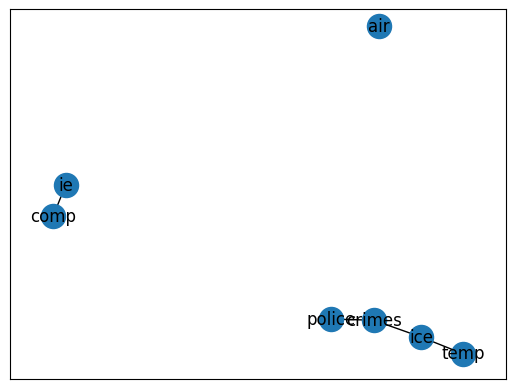
\includegraphics[width=\FigWidth]{figures/practice/chapter-7/sem11-cell43-out0.png}
\caption{Семинар~11: вилка, $Y$ vs $X$. Обратите внимание на сильную связь без учёта $Z$.}
\label{fig:p7-fork1}
\end{figure}
\begin{figure}[htbp]
\centering
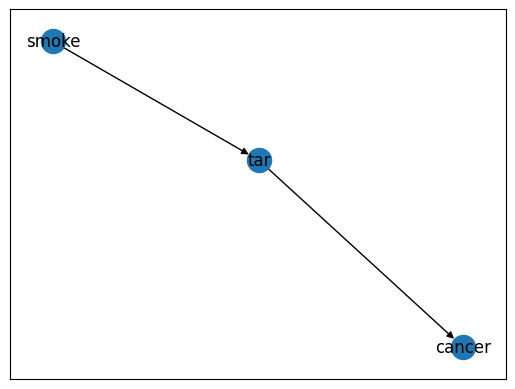
\includegraphics[width=\FigWidth]{figures/practice/chapter-7/sem11-cell51-out0.png}
\caption{Семинар~11: вилка, $Y$ vs $X+Z$. На графике видно ослабление коэффициента при $X$.}
\label{fig:p7-fork2}
\end{figure}
\medskip\noindent\textbf{Три вопроса.} \textit{Постановка:} симуляция DAG-вилки. 
\textit{Применимость:} регрессия не заменяет $do(X)$; блокировать $Z$. 
\textit{Вывод:} маргинальный коэффициент вводит в заблуждение.\medskip

\paragraph{Коллайдер (sem11).}
$X$ и $Y$ независимы, но при отборе $|Z|>c$ появляется ложная корреляция.
\begin{figure}[htbp]
\centering
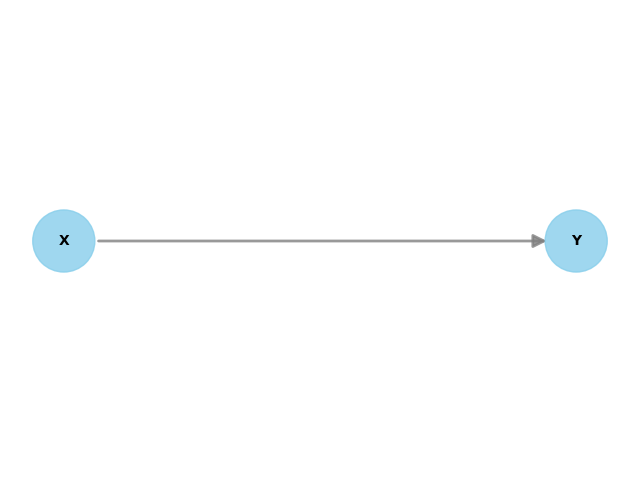
\includegraphics[width=\FigWidth]{figures/practice/chapter-7/sem11-cell61-out2.png}
\caption{Семинар~11: коллайдер. Обратите внимание на корреляцию в подвыборке при $|Z|>c$.}
\label{fig:p7-coll}
\end{figure}
\medskip\noindent\textbf{Три вопроса.} \textit{Постановка:} $X\perp Y$, отбор по коллайдеру $Z$. 
\textit{Применимость:} не включать $Z$ в критерий задней двери (KЗД); объяснять selection bias. 
\textit{Вывод:} условная зависимость --- артефакт отбора.\medskip

\paragraph{Brown, HMM без учителя (sem12).}
Баум--Уэлх на подкорпусе Brown: лог-правдоподобие растёт до плато. Матрица $A$ (рис.~\ref{fig:p7-hmm-trans}).
\begin{figure}[htbp]
\centering
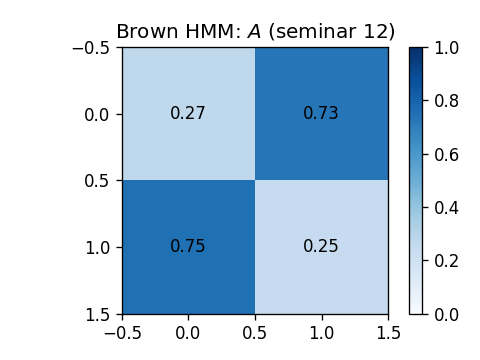
\includegraphics[width=\FigWidth]{figures/practice/chapter-7/sem12-brown-trans-unsupervised.png}
\caption{Семинар~12: матрица $A$ (unsupervised). На графике видно различие диагоналей.}
\label{fig:p7-hmm-trans}
\end{figure}
\medskip\noindent\textbf{Три вопроса.} \textit{Постановка:} символы Brown, скрытые состояния. 
\textit{Применимость:} EM до плато; смотреть $A$, не только LL. 
\textit{Вывод:} метки состояний произвольны, сравнивать с supervised.\medskip

\paragraph{Brown, HMM с разметкой.}
$A$, $B$ по частотам на размеченном корпусе; сравнение с unsupervised --- иная интерпретация состояний, тот же Витерби.
\medskip\noindent\textbf{Три вопроса.} \textit{Постановка:} размеченный vs скрытый HMM. 
\textit{Применимость:} supervised --- частоты; unsupervised --- EM. 
\textit{Вывод:} декодирование одно, интерпретация состояний разная.\medskip

\paragraph{Языковая модель (корпус Jack).}
$n$-граммы, $\chi^2$, перплексия, сглаживание Лапласа; частоты (рис.~\ref{fig:p7-jack-freq}).
\begin{figure}[htbp]
\centering
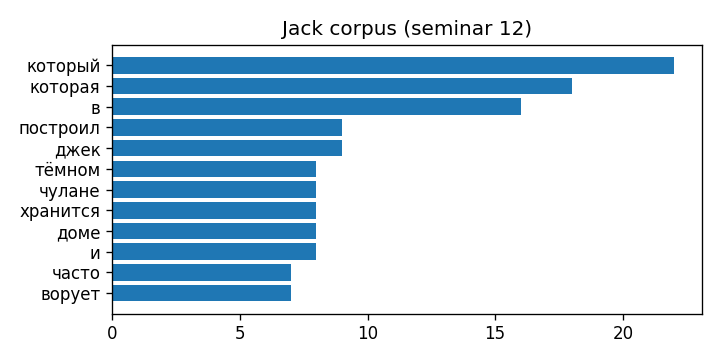
\includegraphics[width=\FigWidth]{figures/practice/chapter-7/sem12-jack-wordfreq.png}
\caption{Семинар~12: частоты слов Jack. Обратите внимание на служебный каркас текста.}
\label{fig:p7-jack-freq}
\end{figure}
\medskip\noindent\textbf{Три вопроса.} \textit{Постановка:} корпус Jack, $n$-граммы. 
\textit{Применимость:} $\chi^2$ на биграммы, перплексия, сглаживание Лапласа. 
\textit{Вывод:} низкая перплексия на повторяющемся тексте не заменяет отложенную выборку (holdout).\medskip

\paragraph{Домашнее sem12.}
Бинарная последовательность по почте: оценить $A$ и сравнить с семинаром.
\medskip\noindent\textbf{Три вопроса.} \textit{Постановка:} своя бинарная цепь. 
\textit{Применимость:} оценка $A$ для двух состояний. 
\textit{Вывод:} сверка с семинарской $A$, не только LL.\medskip

По итогам: DAG и регрессия; HMM --- EM, $A$, $B$; LM --- перплексия и сглаживание.

\section{Контрольные вопросы по теме}

\begin{enumerate}
    \item Объясните парадокс Симпсона на примере лекарства и пола.
    \item Почему в примере~2 (давление) KЗД по $Z$ неверен?
    \item Приведите пример вилки и объясните, почему $Y\perp Z\mid X$.
    \item Запишите формулу задней двери и роль балла включения.
    \item Как PC-алгоритм ориентирует v-структуру $A\to C\leftarrow B$?
    \item Сформулируйте $H_0$ в тесте Грейнджера и статистику $F$.
    \item Вычислите $\mathbb{E}T_i$ для $P_{ii}=0{,}8$.
    \item Для «Дом, который построил Джек» почему перплексия низкая
          без отложенной выборки?
    \item Запишите рекурсию прямого хода и отличие Витерби от $\gamma_t(i)$.
    \item Как устроен M-шаг Баума--Уэлча для $a_{ij}$?
    \item Опишите HMM для разметки частей речи. Что в $A$, что в $B$?
    \item Почему коллайдер нельзя включать в KЗД-множество?
    \item Почему $\sum_j a_{ij}=1$ для каждой строки $i$?
    \item Как изменится $A$ при увеличении \texttt{max\_iterations}?
    \item Сравните лог-правдоподобие на обучении и на отложенной выборке отрезка. Нужна ли большая $n$?
\end{enumerate}
